\documentclass{article}
\usepackage[utf8]{inputenc}
\usepackage{circuitikz}
\usepackage{url}
\usepackage{collectbox}
\usepackage{multirow}
\usepackage{graphicx}
\usepackage{enumerate}
\usepackage{pgfplots}
\usepgfplotslibrary{polar}
\usepgflibrary{shapes.geometric}
\usetikzlibrary{calc}
\usepackage{bondgraphs}
\usepackage{commath}
\usepackage{physics}
\usepackage{comment}
\usepackage{tikz}
\usetikzlibrary{arrows,shapes,   calc, patterns,decorations.pathmorphing,decorations.markings}
\usetikzlibrary{calc,patterns,decorations.pathmorphing,decorations.markings}
\usepackage{amsmath}
\usepackage{amssymb}
\usepackage{mathptmx} % assumes new font selection scheme installed
\usepackage{natbib}        % required for bibliography
\newtheorem{definition}{Definition}

\definecolor{darkgreen}{rgb}{0, 0.4961, 0}
\title{New Bicomplex Hamiltonian}
\author{ }
\date{August 2022}

\begin{document}

\maketitle

\include{Sections/Introduction}
\include{Sections/Background}
\section{Hamiltonian on Special Complex Product Manifolds}

\section{Our Proposal: Strictly Symplectic Bicomplex Hamiltonian Systems }
\label{sec: bicomplex}
In this section, we introduce what we call ``bicomplex Hamiltonian systems''.  These will be seen to adhere strictly the three requirements ((i)-(iii)) for a Hamiltonian system, while incorporating any dissipation that may be present.

To this end, we write the dynamics of a bicomplex Hamiltonian systems as
\begin{equation}
\label{eq: bicomphamdes}
    \Dot{\chi}=\mathcal{J}\nabla\mathcal{H}(\chi),
\end{equation}
which is manifestly in strict Hamiltonian form.  The state variable $\chi$ will take values in $\mathcal{\chi}\in\mathbb{C}^{2}$, hence our choice of bicomplex.  Section \ref{sec: state} shows how the bicomplex state $\chi$  relates to the usual state $x \in \mathbb{R}^{2}$. In Section \ref{sec: struc} we introduce the symplectic structure  matrix $\mathcal{J}$.  Finally, in Section \ref{sec: ham} we derive a
complex Hamiltonian function $\mathcal{H}(\chi) : \mathbb{C}^{2} \to \mathbb{C}$ on the bicomplex state space.

\subsection{Special complex product manifold}



\subsection{Bicomplex State-Space}
\label{sec: state}
We start from the symplectic manifold $M$ that is endowed with a symplectic structure expressed in local Darboux coordinates as
\begin{equation}
    \omega = \sum_{j=1}^n\dif q_j \wedge \dif p_j
\end{equation}
The symplectic manifold possesses an almost complex structure defined by \cite{}
\begin{equation}
    J_0(\pdv{}{q_j})=\pdv{}{p_j},\hspace{5mm}J_0(\pdv{}{p_j})=-\pdv{}{q_j},
\end{equation}
where $J_0^2=-$Id.
The structure coordinates resulting from this structure are
\begin{equation}
\label{eq: lad}
    \textbf{x}_j =\frac{1}{\sqrt{2}} \left(q_j+i p_j\right),
\end{equation}


Let us consider a define complex states $\textbf{x}_j$ and $\bar{\textbf{x}}_j$ as follows

\begin{equation}
\label{eq: lad}
    \textbf{x}_j =\frac{1}{\sqrt{2}} \left(q_j+i p_j\right),
\end{equation}
and
\begin{equation}
\label{eq: ladc}
    \bar{\textbf{x}}_j = \frac{1}{\sqrt{2}}\left(q_j-ip_j\right)
\end{equation}



 \begin{align}
\label{eq: q}
    q &= \frac{1}{\sqrt{2}}(\bar{\textbf{x}}+\textbf{x}),\\
\label{eq: p}    
    p &= \frac{i}{\sqrt{2}}(\bar{\textbf{x}}-\textbf{x})
\end{align}

\begin{align}
    \frac{\textbf{x}^2+\bar{\textbf{x}}^2}{2} &= \frac{1}{2}(q^2-p^2)\\
    \textbf{x}\bar{\textbf{x}} &=\frac{1}{2} p^2+q^2\\
     i \frac{\textbf{x}^2-\bar{\textbf{x}}^2}{2} &= qp
\end{align}


\begin{comment}
Here $\omega=\sqrt{1/IC}$ is the generalized natural frequency, $I$ is the generalized inertance, and $C$ is the generalized compliance.
Some domain specific examples of inertances and compliances are listed in Table \ref{tb:elements}.
\begin{table}[h]
\caption{{\small Elements}}
\label{tb:elements}
\begin{center}
\begin{tabular}{lll}
\hline
\textbf{Generalized} & \textbf{Mechanical} & \textbf{Electrical} \\ \hline
Compliance, $C$      & Spring, $1/k$       & Capacitor, $C$      \\
Inertance, $I$       & Mass, $m$           & Inductor, $L$       \\
Resistance, $r$      & Damper, $b$         & Resistor, $R$       \\ \hline
\end{tabular}
\end{center}
\end{table}
\end{comment}















To define the bicomplex state $\chi$, let
 $\textbf{x} =\begin{bmatrix}
\textbf{x}_1,\dots,\textbf{x}_n
\end{bmatrix}^\intercal$ and $\bar{\textbf{x}} =\begin{bmatrix}
\bar{\textbf{x}}_1,\dots,\bar{\textbf{x}}_n
\end{bmatrix}^\intercal$ and set 
\begin{equation}
\label{eq: state}
    \chi = \begin{bmatrix}
    \textbf{x}& \Bar{\textbf{x}}
    \end{bmatrix}^\intercal
\end{equation}
 We can consider the bicomplex state as a conjugate pair, for instance by thinking of $\textbf{x}$ as the generalized complex positions and $\bar{\textbf{x}}$ as the conjugate generalized complex momenta. The bicomplex state is an element of $\mathbb{C}^{2n}$ and clearly even-dimensional, thus meeting requirement (i).



%\begin{table}[h]
%\caption{{\small Variables}}
%\label{tb:variables}
%\centering
%\begin{tabular}{lll}
%\hline
%\textbf{Generalized} & \textbf{Mechanical} & \textbf{Electrical}     \\ \hline
%Momentum, $p$        & Momentum, $p$       & Flux Linkage, $\phi$ \\
%Position, $q$        & Position, $q$       & Charge, $q$             \\
%Effort, $e$          & Force, $F$          & Voltage, $V$            \\
%Flow, $f$            & Velocity, $v$       & Current, $I$            \\ \hline
%\end{tabular}
%\end{table}

\subsection{Almost Complex Structures}
The standard symplectic manifold on the phase space $\mathbb{R}^2n$ is endowed with the standard symplectic structure
\begin{align*}
    \omega_0 &= \sum \dif q \wedge \dif p,
\end{align*}
standard inner product
\begin{equation*}
    g_0 &= \langle \cdot , \cdot \rangle
\end{equation*}
if we identify pairs $(q_j, p_j)$ with the complex state $\textbf{x}_j = q_j+ip_j$, multiplication by $i$ induces a constant linear map $J_0$ on the tangent spaces of $\mathbb{R}^{2n}$ [Cannas da Siva]


\subsection{Kahler Manifolds}
\label{sec: kahler}
Consider a complex manifold $M$ with a compatible symplectic form $\omega$, on a local chart $(\mathcal{U}, \textbf{x}_1,\dots,\textbf{x}_n)$ given by
\begin{equation}
    \omega = \frac{i}{2}\sum_{j,k=1}^n h_{jk}\dif \textbf{x}_j \wedge \dif \bar{\textbf{x}}_j,
\end{equation}



\subsection{Bicomplex Symplectic Structure}
\label{sec: struc}
The bicomplex state space is endowed with a bicomplex Poisson bracket (see e.g. \cite{NOVAES2004})
\begin{equation}
\label{eq:PoissonBracket}
\{\mathcal{U},\mathcal{V}\} =
-i \begin{bmatrix}
    \frac{\partial \mathcal{U}}{\partial \textbf{x}}&\frac{\partial \mathcal{V}}{\partial \bar{\textbf{x}}} 
    -
        \frac{\partial \mathcal{V}}{\partial \textbf{x}}&\frac{\partial \mathcal{U}}{\partial \bar{\textbf{x}}} 
    \end{bmatrix}
\end{equation}
Here $\mathcal{U}(\chi)$ and $\mathcal{V}(\chi)$ are holomorphic functions on the bicomplex state space.  




From this Poisson bracket we can reverse-engineer the symplectic structure matrix $\mathcal{J}$ (see \cite[p.~65]{marsden}).  In general, 
\begin{equation}
\label{eq: comppois}
    \{\mathcal{U},\mathcal{V}\} = \begin{bmatrix}
    \frac{\partial \mathcal{U}}{\partial \textbf{x}}&\frac{\partial \mathcal{U}}{\partial \bar{\textbf{x}}}
    \end{bmatrix} 
\mathcal{J}
    \begin{bmatrix}
    \frac{\partial \mathcal{V}}{\partial \textbf{x}}\\
    \frac{\partial \mathcal{V}}{\partial \bar{\textbf{x}}}
    \end{bmatrix},
    %=d\mathcal{U}\cdot \mathcal{B}\nabla \mathcal{V}
\end{equation}
and comparing this with (\ref{eq:PoissonBracket}), we see that
\begin{equation}
\label{eq: structure}
    \mathcal{J}= \begin{bmatrix}
    0&-i\\i&0
    \end{bmatrix}
\end{equation}
We can check that $\mathcal{J}$ is symplectic by taking the skew-symmetric
\begin{equation*}
    \Omega = \begin{bmatrix}
    0&-1\\1&0
    \end{bmatrix},
\end{equation*}
and verifying that  
\begin{equation}
    \mathcal{J}^\dagger\Omega\mathcal{J}=\Omega,
\end{equation}
and that det$(\mathcal{J})=-1$. %Why is this important?
Here $\mathcal{J}^\dagger$ is the conjugate transpose of $\mathcal{J}$.  This completes requirement (ii).


%For a Hamiltonian system and any function $A(x)$, the Poisson bracket has the property 
%\begin{equation*}
%    \dot{A}=\{A,H\}
%\end{equation*}

%Writing the time-evolution of the generalized positions and momenta in terms of the Poisson bracket results in Hamilton's equations
%\begin{equation*}
%    \dot{q}=\{q,H\}=\frac{\partial H}{\partial p}
%\end{equation*}
%and
%\begin{equation*}
%    \dot{p}=\{p,H\} = -\frac{\partial H}{\partial q}
%\end{equation*}
%Collecting the two Hamilton's equations and writing them in matrix form, results in the Hamiltonian system in (\ref{eq: Hamiltonianmech}).
%From this, it can be readily derived that $J$ is the following symplectic matrix




%In the state-space coordinates $\chi$ we derive that the Poisson bracket of two functions $A(\chi)$ and $B(\chi)$ takes the form

%We define the time-evolution of the ladder state $a\in\mathbb{C}^n$ as the Poisson bracket of $a$ and a complex Hamiltonian $\textbf{H}\in \mathbb{C}^n$
%\begin{equation}
%\label{eq: ham1}
%    \dot{a}\ = \{a,\textbf{H} \} = -i\frac{\partial {\textbf{H}}}{\partial \bar{a}}
%\end{equation}
%By complex conjugation we immediately get that the time-evolution of the conjugate ladder state $\bar{a}$ is
%\begin{equation}
%\label{eq: ham2}
%    \dot{\bar{a}} = \overline{\{a,\textbf{H} \}}=\{\bar{a},\bar{\textbf{H}}\}= i\frac{\partial \bar{\textbf{H}}}{\partial a}
%\end{equation}
%Equations (\ref{eq: ham1}) and (\ref{eq: ham2}) fully define the dynamics of a system with state $\chi=\begin{bmatrix}
%a&\bar{a}
%\end{bmatrix}^\intercal$.
%Therefore, we can collect these two equations and put write them in the desired matrix form given in (\ref{eq: bicomphamdes}).
%The resulting system is 
%\begin{equation}
%\label{eq:  dynamics}
%    \dot{\chi}=\begin{bmatrix}
%    \dot{a} \\ \dot{\bar{a}}
%    \end{bmatrix}=\begin{bmatrix}
%    0&-i\\i&0
%    \end{bmatrix}
%    \begin{bmatrix}
%    \partial\bar{\textbf{H}}/{\partial a}\\
%    \partial\textbf{H}/\partial\bar{a}
%    \end{bmatrix}
%\end{equation}
%Here, the so-called \textit{naive gradient} \cite[p~64]{marsden} of the bicomplex Hamiltonian $\mathcal{H} \in \mathbb{C}^{2n}$ is $\nabla \mathcal{H} = \begin{bmatrix}
%    \partial\bar{\textbf{H}}/{\partial a}&
%    \partial\textbf{H}/\partial\bar{a}
%    \end{bmatrix}^\intercal$.



%Some attentive readers may note that for matrices with complex-valued entries the condition for a symplectic matrix is sometimes given as \cite{XU20031}
%\begin{equation}
%\label{eq: conjsym}
%    J^\dagger\Omega J=\Omega,
%\end{equation}
%where $J^\dagger$ is the conjugate transpose of $J$. 
%To distinguish them from real-valued symplectic matrices, some authors refer to matrices that satisfy (\ref{eq: conjsym}) as conjugate symplectic matrices \cite{conjsymp}.  
%Although $\mathcal{J}$ also satisfies (\ref{eq: conjsym}), we will stick to the term symmetric matrix.



%which in matrix form can be written as
%\begin{equation}
%\label{eq: bracket}
%\begin{split}
%    \{A,B\} &= \frac{\partial^\intercal A}{\partial \chi}\mathcal{J}\frac{\partial B}{\partial \chi},
%\end{split}
%\end{equation}
%In this matrix notation, $\mathcal{J}$ denotes the following conjugate symplectic\footnote{see (\cite{symplectic})} matrix
%\begin{equation}
%    \mathcal{J}=\begin{bmatrix}
%    0 &-i\\i&0
%    \end{bmatrix}
%\end{equation}

%With the Poisson bracket in (\ref{eq: bracket}) it can be verified that the state-space $\chi$ is canonical by checking that $\{a,a\} = 0$, $\{\bar{a},\bar{a}\}=0$, and $\{a,\bar{a}\}=-i\delta$.
 


\subsection{Complex Hamiltonian}
\label{sec: ham}

%%I'm going to put some motivation here.  we need to remark that for a function to be Hamiltonian, we need it to be the generator of the time translation etc.
For a function $\mathcal{H}$ to be a Hamiltonian, it should give the time derivative of a function under the Poisson bracket.  
In particular, using the bracket (\ref{eq:PoissonBracket}) for the complex position $\textbf{x}$ requires that 
\begin{equation}
\label{eq:Poissonx}
    \dot{\textbf{x}}=\{\textbf{x},\mathcal{H}\}= -i\frac{\partial\mathcal{H}}{\partial \bar{\textbf{x}}}
\end{equation}
Although the complex conjugate momentum $\bar{\textbf{x}}$ is not holomorphic, it is nevertheless readily found by complex conjugating the above expression that
\begin{equation}
\label{eq:Poissonxbar}
    \dot{\bar{\textbf{x}}}=\overline{\{\textbf{x},\mathcal{H}\}}=i\frac{\partial \bar{\mathcal{H}}}{\partial \textbf{x}}
\end{equation}
If we collect $\dot{\textbf{x}}$ and $\dot{\bar{\textbf{x}}}$ into a single expression for $\dot{\chi}$ and
express the bicomplex gradient as 
\begin{equation}
\label{eq:BicomplexGradient}
    \nabla \mathcal{H}(\chi) \triangleq \begin{bmatrix}
    \frac{\partial {\bar{\mathcal{H}}}}{\partial \textbf{x}} &\frac{\partial {\mathcal{H}}}{\partial \bar{{\textbf{x}}}}
    \end{bmatrix}^\intercal,
\end{equation}
we can summarize the dynamics in a strictly symplectic manner as $\Dot{\chi}=\mathcal{J}\nabla\mathcal{H}(\chi)$.
 This reproduces (\ref{eq: bicomphamdes}) and completes our determination of a strictly symplectic bicomplex Hamiltonian System.
 
 \subsection{Casimirs}
\label{sec:Casimirs}
The complex Hamiltonian itself is finally found by integrating  expression (\ref{eq:BicomplexGradient}).  However, this determines the Hamiltonian up to an integrating constant, so there will be freedom of choice in choosing a Hamiltonian.  

To determine the nature of such an integrating constant, notice that
evidently a  function $\mathcal{C}$ that gives 0 under the Poisson bracket can be added to the Hamiltonian for an alternate Hamiltonian $\mathcal{K} = \mathcal{H} + \mathcal{C}$.
This addition does not affect the motion since
\begin{equation}
    \{\textbf{x},\mathcal{K}\} = \{\textbf{x},\mathcal{H}\} 
    + \{\textbf{x}, \mathcal{C}\} = \dot{\textbf{x}} + 0 = \dot{\textbf{x}}
\end{equation}
Functions such that $\{ \mathcal{U},\mathcal{C} \} = 0$  for any  function $\mathcal{U}$ are known as Casimir functions. This can be used to advantage in closed-loop systems as we show in Section \ref{sec: control} for bicomplex systems. 


\section{Application: The Damped Harmonic Oscillator}
\label{sec: dho}
In practice, the real-valued dynamics of a system in the $A$-matrix representation are known. 
In this section we show how this is used to determine the complex Hamiltonian (up to a Casimir) for the case of the damped harmonic oscillator (DHO).  

Our strategy is to determine the bicomplex $\mathcal{A}$-matrix corresponding to the usual $A$-matrix and then to integrate $\mathcal{A}\chi = \mathcal{J}\nabla \mathcal{H}$.

%In this section, we show how the damped harmonic oscillator (DHO) can be described as a bicomplex Hamiltonian system.  We do this for two configurations of the DHO: a series RLC circuit (Figure \ref{fig:series}) and  a parallel RLC circuit (Figure \ref{fig:parallel}).
%We refer to the first configuration as the series DHO and to the second configuration as the parallel DHO.

\subsection{DHO}
\label{sec: DHO}
Consider the system in Figure \ref{fig:series}.
We start with the familiar state-space representation on $\mathbb{R}^{2}$ spanned by the position (or charge) $q$ and momentum (or flux linkage) $p$
\begin{equation}
\label{eq: dynAx}
    \underbrace{\begin{bmatrix}
    \dot{q}\\
    \dot{p}
    \end{bmatrix}}_{\dot{x}}=\underbrace{\begin{bmatrix}
    0 &1/I\\
    -1/C &-{r}/{I}
    \end{bmatrix}}_{A}\underbrace{
    \begin{bmatrix}
    q\\p
    \end{bmatrix}}_{x}
\end{equation} 

To convert this into a state-space representation on $\mathbb{C}^{2}$
\begin{equation}
    \dot{\chi} = \mathcal{A} \chi ,
\end{equation}
%conform Equation \ref{eq: bicomphamdes}.
%\begin{equation}
 %   \dot{\chi}=\mathcal{J}\nabla\mathcal{H}_p(\chi)
%\end{equation}
invert the expressions for the complex states (\ref{eq: lad}) and (\ref{eq: ladc}) to recover
 \begin{align}
\label{eq: q}
    q &= (\bar{\textbf{x}}+\textbf{x})/2,\\
\label{eq: p}    
    p &= i(\bar{\textbf{x}}-\textbf{x})/2,
\end{align}
 substitute these into (\ref{eq: dynAx}) and rearrange to obtain
%Substituting (\ref{eq: q}) and (\ref{eq: p}) in the right-hand side of (\ref{eq: dynAx}) and the time derivatives of (\ref{eq: q}) and (\ref{eq: p}) in the left-hand side of (\ref{eq: dynAx}) yields
%\begin{equation}
 %   \begin{bmatrix}
  %  \sqrt{\frac{1}{2I\omega}}(\dot{\bar{a}}+\dot{a})\\
   %  i\sqrt{\frac{I\omega}{2}}(\dot{\bar{a}} -\dot{a})
    %\end{bmatrix}=
    %\begin{bmatrix}
    %0 &1/I\\
    %-1/C &-{R}/{I}
    %\end{bmatrix}
    %\begin{bmatrix}
    % \sqrt{\frac{1}{2I\omega}}(\bar{a}+a)\\
    % i\sqrt{\frac{I\omega}{2}}(\bar{a}-a)
%    \end{bmatrix}
%\end{equation}
%By rearranging this system of equations, we obtain the dynamics of the DHO
%Substituting these inverted definitions in (\ref{eq: dynAx}) results (after some rearranging) in the corresponding bicomplex state-space representation
\begin{equation}
\label{eq: achi}
    \underbrace{\begin{bmatrix}
    \dot{\textbf{x}}\\\dot{\bar{\textbf{x}}}
    \end{bmatrix}}_{\dot{\chi}}=\underbrace{ \begin{bmatrix}
    -(\beta+i\phi) &\beta-i\alpha\\
    \beta+i\alpha  &-(\beta-i\phi) 
    \end{bmatrix}}_{\mathcal{A}}
    \underbrace{\begin{bmatrix}
    \textbf{x}\\\bar{\textbf{x}}
    \end{bmatrix}}_{\chi},
\end{equation}
where $\alpha=  (1/2C-1/2I)$, $\phi= (1/2C+1/2I)$ and $\beta=r/(2I)$ is the damping coefficient. %\footnote{ Here, the subscript $s$ stands for the series configuration of the RLC circuit in Fig. \ref{fig:series}, distinguishing it from DHO in Fig. \ref{fig:parallel}.} 
Clearly, this $\mathcal{A}$-matrix is part of $SU(1,1)$.




To express the dynamics in bicomplex pH form (\ref{eq: bicomphamdes}), we set
$$ \mathcal{J}\nabla \mathcal{H}=\mathcal{A}\chi ,
$$
 substitute for the $\mathcal{A}$-matrix in (\ref{eq: achi}) and  evaluate the left-hand side using the bicomplex symplectic matrix (\ref{eq: structure}) and gradient (\ref{eq:BicomplexGradient}), to obtain
\begin{equation}
\label{eq:Partial1}
      -i\frac{\partial \mathcal{H}}{\partial \bar{\textbf{x}}} =  -(\beta+i\phi)\textbf{x} +(\beta-i\alpha)\bar{\textbf{x}},
\end{equation}
\begin{equation}
\label{eq:Partial2}
  i\frac{\partial \bar{\mathcal{H}}}{\partial {\textbf{x}}} =  (\beta+i\alpha)\textbf{x} -(\beta-i\phi)\bar{\textbf{x}},
\end{equation}
conform the expressions for the Poisson brackets in (\ref{eq:Poissonx}) and (\ref{eq:Poissonxbar}).  

Integrating, we find the following expression for the complex Hamiltonian
\begin{equation}
\label{eq: cham}
   \mathcal{H} = \alpha \frac{\textbf{x}^2 +\bar{\textbf{x}}^2}{2}
    +(\phi-i\beta)\textbf{x}\bar{\textbf{x}}-{i{\beta}\frac{\textbf{x}^2-\bar{\textbf{x}}^2}{2}}
\end{equation}
Its validity is readily checked by substituting into (\ref{eq:Partial1}) and (\ref{eq:Partial2}).


\begin{figure}
    \centering
    \includegraphics[width=0.8\linewidth]{flow.png}
    \caption{{\small The Bicomplex Hamiltonian flow consists of three parts: a rotation with orbits by $\omega\textbf{x}\bar{\textbf{x}}$ (green), a contraction with orbits $-i\beta^{{}^+}\textbf{x}\bar{\textbf{x}}$ (blue), and a squeeze with orbits $-i\beta^{{}^-} (\frac{\textbf{x}^2-\bar{\textbf{x}}^2}{2})$ (red). The solid line represents a composite flow. The direction of the squeeze flow reverses with the sign of $\beta^{{}^-}$.}}.  
   \label{fig: vec}
\end{figure}
%and 
%\begin{equation}
%    \bar{\textbf{H}}_s = (\omega-i\beta_s )\textbf{x}\bar{\textbf{x}}+i\frac{\beta_s}{2}\bar{\textbf{x}}^2
%\end{equation}
%Here, $\kappa_s$ is chosen so that ${\textbf{H}_s}$ and $\bar{\textbf{H}_s}$ are bilinear functions of both complex state-variables $\textbf{x}$ and $\bar{\textbf{x}}$.
%Notice that $\bar{\textbf{H}}_s$ is indeed the complex conjugate of $\textbf{H}$.

%Substituting the derived bicomplex Hamiltonian  $\mathcal{H}_s$ in (\ref{eq: bicomphamdes}), we find that the DHO can indeed be modeled as a Hamiltonian system.


\begin{figure}[t]
        \begin{circuitikz}[/tikz/circuitikz/bipoles/length=1cm,scale=0.7]
        \draw    (0,1.5)
            to[american inductor=$I$ ] (4,1.5) 
            to[C=$C$] (4,0)
            to[R=$r$] (0,0);
        \end{circuitikz} %[\abovecaptionskip]
    %\small (a) Electrical series RLC circuit
        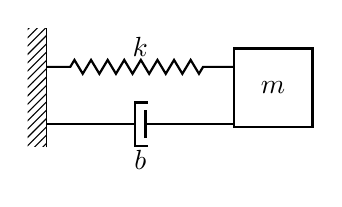
\begin{tikzpicture}[scale=0.1]
             \tikzstyle{spring}=[thick,decorate,decoration={zigzag,pre length=0.3cm,post length=0.3cm,segment length=6}]
             \tikzstyle{damper}=[thick,decoration={markings,  
              mark connection node=dmp,
              mark=at position 0.5 with 
             {
                    \node (dmp) [thick,inner sep=0pt,transform shape,rotate=-90,minimum width=15pt,minimum height=3pt,draw=none] {};
               \draw [thick] ($(dmp.north east)+(1pt,0)$) -- (dmp.south east) -- (dmp.south west) -- ($(dmp.north west)+(1pt,0)$);
                \draw [thick] ($(dmp.north)+(0,-5pt)$) -- ($(dmp.north)+(0,5pt)$);
              }
            }, decorate]
            \tikzstyle{ground}=[fill,pattern=north east lines,draw=none,minimum width=0.755cm,minimum height=0
            cm]
            \begin{scope}[xshift=5cm]
            \node [style={draw,outer sep=0pt,thick}] (M)  [minimum width=1cm, minimum height=1cm] {$m$} ;
            \node (wall) [ground, rotate=-90, minimum width=1.5cm,yshift=-3cm] {};
            \draw (wall.north east) -- (wall.north west);
                        \draw [spring] (wall.155) -- ($(M.north west)!(wall.155)!(M.south west)$) node [midway,above] {$k$};
            \draw [damper] (wall.15) -- ($(M.north west)!(wall.15)!(M.south west)$)node [midway,below=0.2] {$b$};
         %   \draw [-latex,ultra thick] (M.east) ++ (0cm,0) -- +(1cm,0) node [right, above] {$F$};
            \end{scope}
         \end{tikzpicture} \\%[\abovecaptionskip]
  \caption{{\small Damped harmonic oscillator with series configuration. The symbols are listed in Table \ref{tb:elements}. This system can be modeled as a Hamiltonian system with complex Hamiltonian in (\ref{eq: cham})} }
  \label{fig:series}
\end{figure}


%Then, we substitute (\ref{eq: achi}) for $\dot{\chi}$ in (\ref{eq:  dynamics}).
%After multiplying both sides of the resulting equation by $\mathcal{J}^{-1}$ this results in
%\begin{equation}
%    \begin{bmatrix}
%    \partial\bar{\textbf{H}}/{\partial a}\\
%    \partial\textbf{H}/\partial\bar{a}
%    \end{bmatrix}= \begin{bmatrix}
%    0&-i\\i&0
%    \end{bmatrix}\begin{bmatrix}
%    -(\beta_s+i\omega) &\beta_s\\
%    \beta_s &-(\beta_s-i\omega) %    \end{bmatrix}
%    \begin{bmatrix}
%    a\\\bar{a}
%    \end{bmatrix}
%\end{equation}


 


%It can be easily verified that in case of zero dissipation ($\beta_s=0$) the Hamiltonian reduces to $\mathcal{H}=\omega a\bar{a}$, which coincides with the classical Hamiltonian $H=p^2/(2m)+k/2q^2$. 
%This case of the complex-valued Hamiltonian has already been established in the literature, see e.g. \cite[p.~194]{corben1994classical}. 


%and
%\begin{equation}
%\label{eq: cham1}
 %   \bar{\textbf{H}}_p = (\omega -i\beta_p)\textbf{x}\bar{\textbf{x}}-i\frac{\beta_p}{2}\bar{\textbf{x}}^2
%\end{equation}
%%Again, substituting this Hamiltonian in (\ref{eq: bicomphamdes}) shows that the parallel DHO can be modeled as a Hamiltonian system.
\begin{figure}[t]
\begin{circuitikz}[/tikz/circuitikz/bipoles/length=1cm,scale=0.7] \draw
          (0,1.5)
          to[american inductor={$I$} ] (2.5,1.5) 
           to[C={$C$}] (2.5,0)
         (2.5,1.5) -- (4,1.5)
           to[R={$r$}] (4,0)
          to[] (0,0)
          (2.5,0) node[ground]{};
        \end{circuitikz} 
        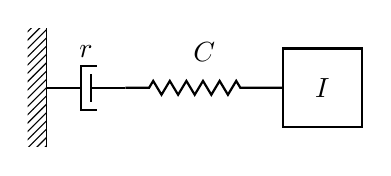
\begin{tikzpicture}
             \tikzstyle{spring}=[thick,decorate,decoration={zigzag,pre length=0.3cm,post length=0.5cm,segment length=6}]
             \tikzstyle{damper}=[thick,decoration={markings,  
              mark connection node=dmp,
              mark=at position 0.5 with 
             {
                    \node (dmp) [thick,inner sep=0pt,transform shape,rotate=-90,minimum width=15pt,minimum height=3pt,draw=none] {};
               \draw [thick] ($(dmp.north east)+(2pt,0)$) -- (dmp.south east) -- (dmp.south west) -- ($(dmp.north west)+(2pt,0)$);
                \draw [thick] ($(dmp.north)+(0,-5pt)$) -- ($(dmp.north)+(0,5pt)$);
              }
            }, decorate]
            \tikzstyle{ground}=[fill,pattern=north east lines,draw=none,minimum width=0.755cm,minimum height=0
            cm]
            \begin{scope}[xshift=9cm]
            %\node [style={draw,outer sep=0pt,thick}] (M)  [minimum width=2cm, minimum height=2cm] {$I: m$} ;
            \node (wall) [ground, rotate=-90, minimum width=1.5cm,yshift=-3cm] {};
            \draw (wall.north east) -- (wall.north west);
           \draw [damper] (wall.north) -- 
          +(1,0)coordinate(t) node [midway,above=0.25] {$r$};
             \draw [spring](t)--
          +(2,0) node [midway,above=0.2] {$C$} node[style={draw,outer sep=0pt,thick}, anchor=west] (M)  [minimum width=1cm, minimum height=1cm] {$I$} ;
         % \draw [-latex,ultra thick] (M.east) ++ (0cm,0) -- +(1cm,0) node [right, above] {$u: F$};
         \end{scope}
         \end{tikzpicture} \\%[\abovecaptionskip]
    %\small (b) Mechanical analog of the parallel RLC circuit
  \caption{{\small Damped harmonic oscillator with parallel configuration. The symbols are defined in Table \ref{tb:elements}.
  This system can be modeled as a Hamiltonian system with complex Hamiltonian in (\ref{eq: cham1})}}
  \label{fig:parallel}
\end{figure}

\subsection{Resistive Configurations}
For the system in  Figure \ref{fig:parallel} with the damper in series with the spring (or resistor in parallel with the capacitor), we can follow the same procedure as in Section \ref{sec: DHO} to find:
\begin{equation}
\label{eq: cham1}
  \mathcal{H} =
  \omega\textbf{x}\bar{\textbf{x}}-i{\beta}\textbf{x}\bar{\textbf{x}}+i\beta(\frac{\textbf{x}^2 -\bar{\textbf{x}}^2}{2})
\end{equation}
For this case the damping coefficient  $\beta = 1/(2rC)$.
A comparison of this Hamiltonian with (\ref{eq: cham}) shows that the only modification is the sign of the rightmost term.  
Physically, this comes about because the  damping is now proportional to the position, instead of to the momentum.

In general, we can consider systems with two resistive elements as combinations of these two extremes.
Combining the Hamiltonians of these extremes, (\ref{eq: cham}) and (\ref{eq: cham1}), we obtain the general complex Hamiltonian of a DHO
\begin{equation}
\label{eq: chamgeneral}
  \framebox{ 
  $\mathcal{H}$ 
  = \stackrel{{\small \color{darkgreen} \text{rotation}}}{\underbrace{\omega\textbf{x}\bar{\textbf{x}}}_{\small \begin{tabular}{l}
       {\small \text{Storage}}\\{\small \text{Function}\  $\mathcal{S}$ }
  \end{tabular}}} -\underbrace{\left( \stackrel{{\color{blue}\text{contraction}}}{i{\beta^{{}^+}}\textbf{x}\bar{\textbf{x}}}+\stackrel{\small {\color{red}\text{squeeze}}}{i\beta^{{}^-}\left(\frac{\textbf{x}^2 -\bar{\textbf{x}}^2}{2}\right)}\right)}_{\small \text{Resistive Function}\  \mathcal{R}}}
\end{equation}
Here $\beta^{{}^+}=(\beta_s+\beta_p)$ and $\beta^{{}^-}=(\beta_s-\beta_p)$ for $\beta_s = r/(2I)$ and $\beta_p= 1/(2rC)$. 
This Hamiltonian is valid for the simple DHO with any resistive configuration. 


\subsection{Geometry of the Complex Hamiltonian Flow}
In equation (\ref{eq: chamgeneral}) we indicate how the  complex Hamiltonian of the DHO can be decomposed into the sum of two functions: an energy storage function $\mathcal{S}$ and a resistive function $\mathcal{R}$.  
Figure \ref{fig: vec} shows the Hamiltonian flows corresponding to these two motions.  

Consider first the storage function.  
In the absence of damping when $\beta^{{}^+}=\beta^{{}^-} = 0$, the complex Hamiltonian reverts to the regular undamped Hamiltonian, since
\begin{equation}
   \omega\textbf{x}\bar{\textbf{x}} =
\frac{1}{2}\frac{p^2}{m} + \frac{1}{2} k q^2,  
\end{equation}
after substituting the expressions for the complex states.  This corresponds to the energy stored in the $C$ and $I$ elements of the system, hence the choice of  storage function for this function.  In the phase plane, the level lines of $\mathcal{S}$ appear as  circles,  shown in green in Figure \ref{fig: vec}.  These circles are precisely the orbits of the rotation group acting on the phase plane giving the familiar Hamiltonian flow of the harmonic oscillator indicated by the green arrow heads.  This flow is symplectic even on $\mathbb{R}^2$. 

The resistive function can be viewed as the sum of two parts: one that appears as a contraction in the phase plane (in blue) and one that appears as a squeeze (in red).
Physically, the contraction models the average dissipation over a cycle, whereas the squeeze provides the dynamics of the  damping within a cycle.
Analyzing the general Hamiltonian shows us that systems with different resistive configurations all share the direction of contraction, but differ in the squeeze. 
In fact, by choosing $\beta_s=\beta_p$, the squeeze disappears altogether and the system follows a smooth hyperbolic spiral down to the equilibrium state.

The orbits of the squeeze map are shown as hyperbolae and these are in fact symplectic on the real phase plane.  
The contraction however compresses the phase volume and therefore cannot be symplectic in $\mathbb{R}^2$.  
This underscores the necessity of using the bicomplex phase space  $\mathbb{C}^2$ to model the dissipation in a symplectic fashion.





\end{document}
